\documentclass{article}
\usepackage[utf8]{inputenc}
\usepackage{graphicx}


\title{Cara Menambahkan aplikasi di apex oracle}

\begin{document}

\maketitle

\section{Pembuatan Aplikasi}

\begin{enumerate}
    \item Langkah pertama, buatlah sebuah data didalam Excell yang nantinya akan di buat dalam apex oracle. seperti contoh diatas
    \begin{figure}[h]
	\centering
		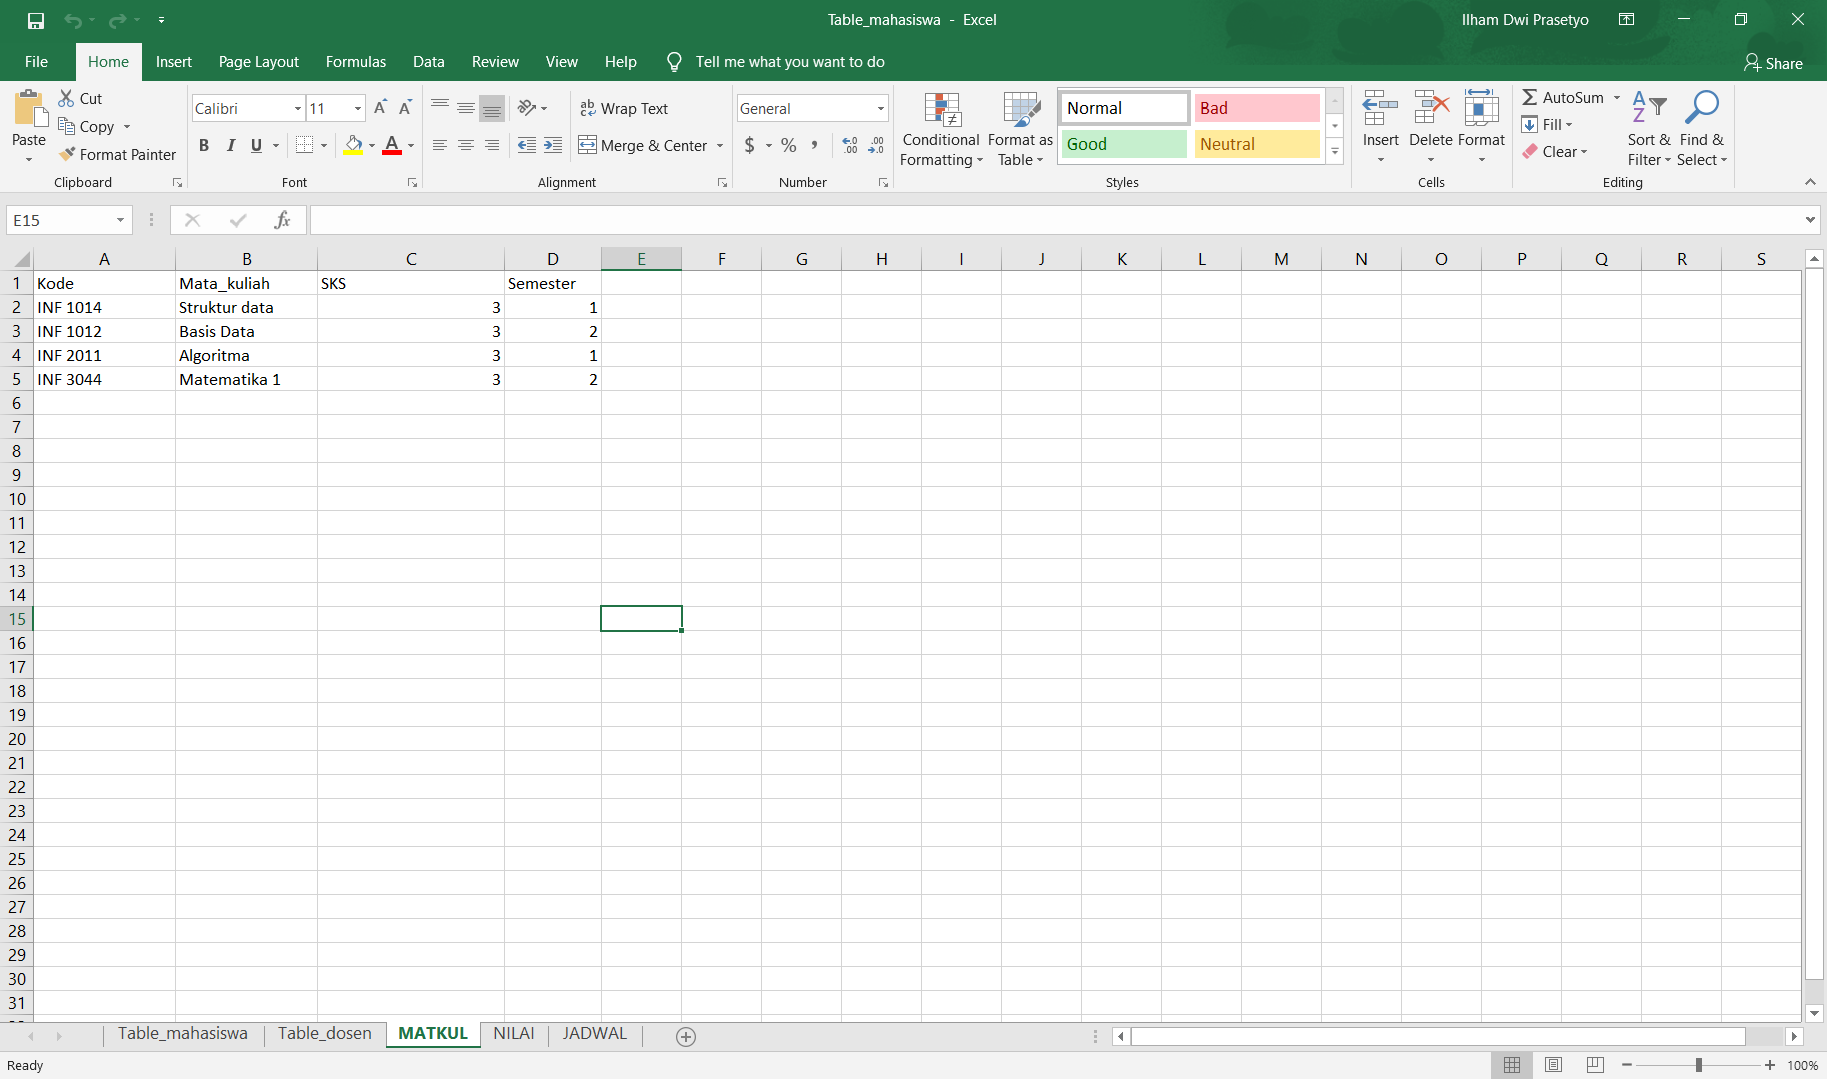
\includegraphics[scale=0.5]{gambar/1.PNG}
		\caption{Data yang Akan di Buat}
\end{figure}
	\item setelah data sudah di buat di excell, lalu buka aplikasi APEX Online dan masuk menggunakan usernamer, workspace dan password yang sudah kita bikin.
	 \begin{figure}[h]
	\centering
		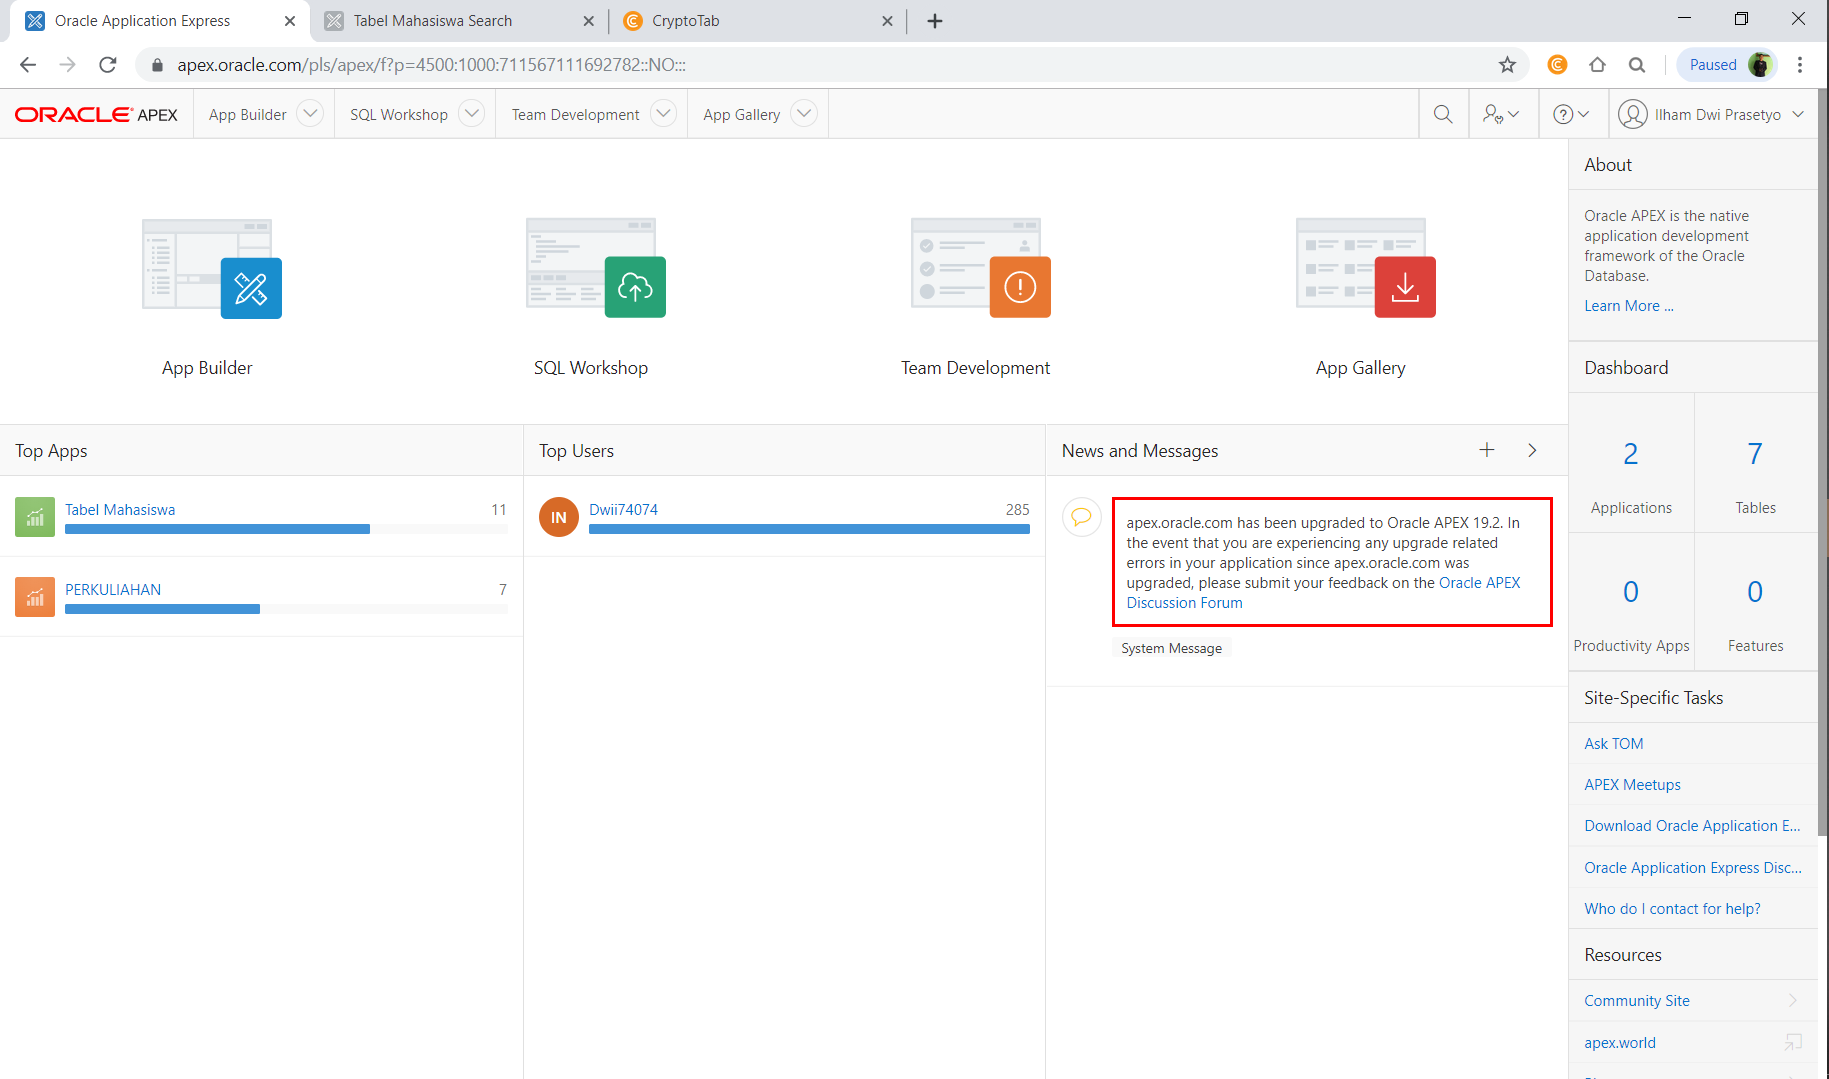
\includegraphics[scale=0.5]{gambar/2.PNG}
		\caption{APEX ONLINE}
\end{figure}
	\item klik App Builder dan akan muncul seperti gambar dibawah:
	 \begin{figure}[h]
	\centering
		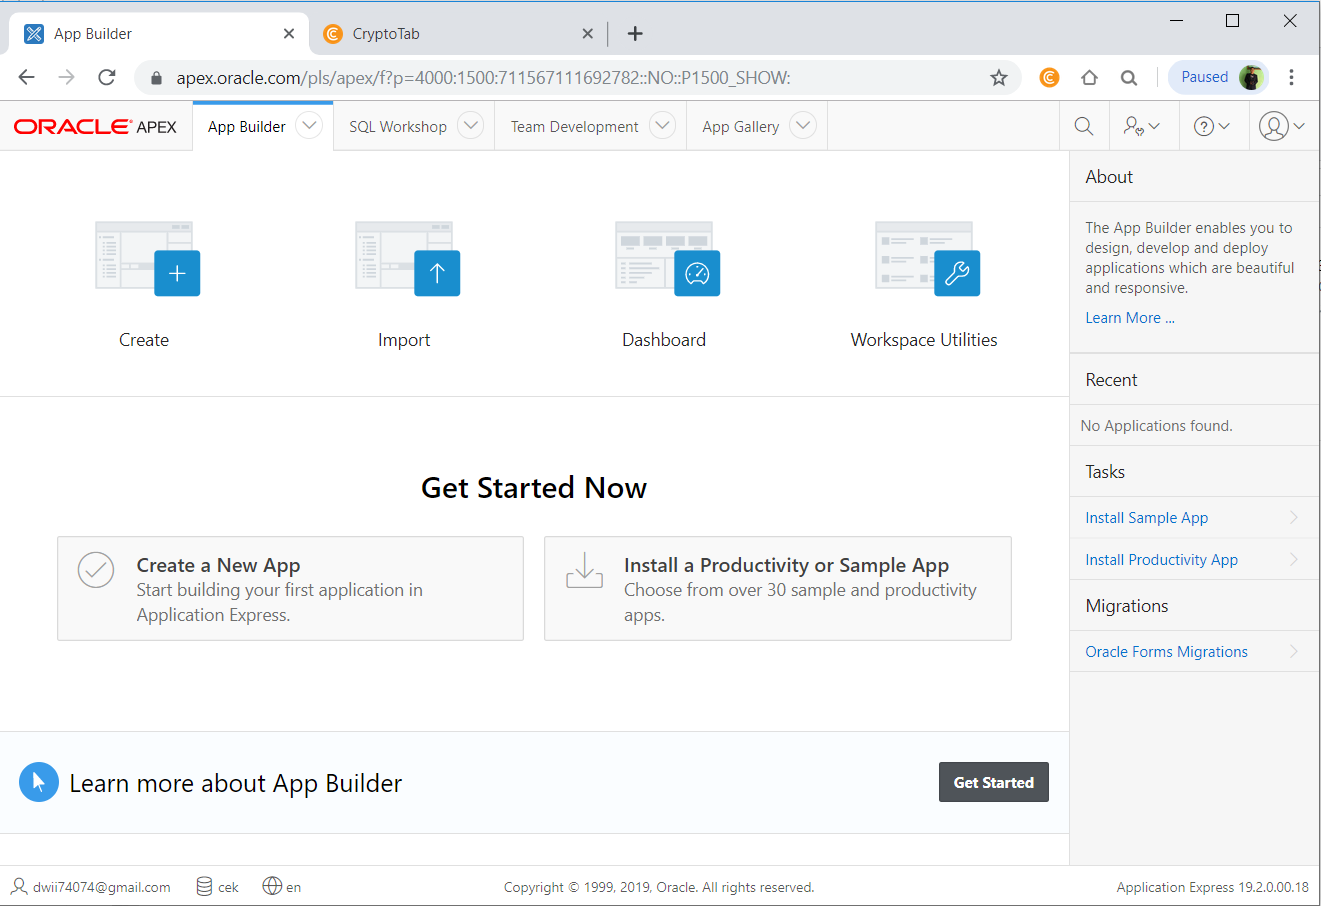
\includegraphics[scale=0.5]{gambar/3.PNG}
		\caption{Tampilan Klik Create}
\end{figure}
\\
\\
\\
\\
\\
\\
\\
\\
\\
\\
\\
\\
\\
\\
	\item Setelah masuk, klik Create dan akan masuk ketampilan dibawah ini :
	 \begin{figure}[h]
	\centering
		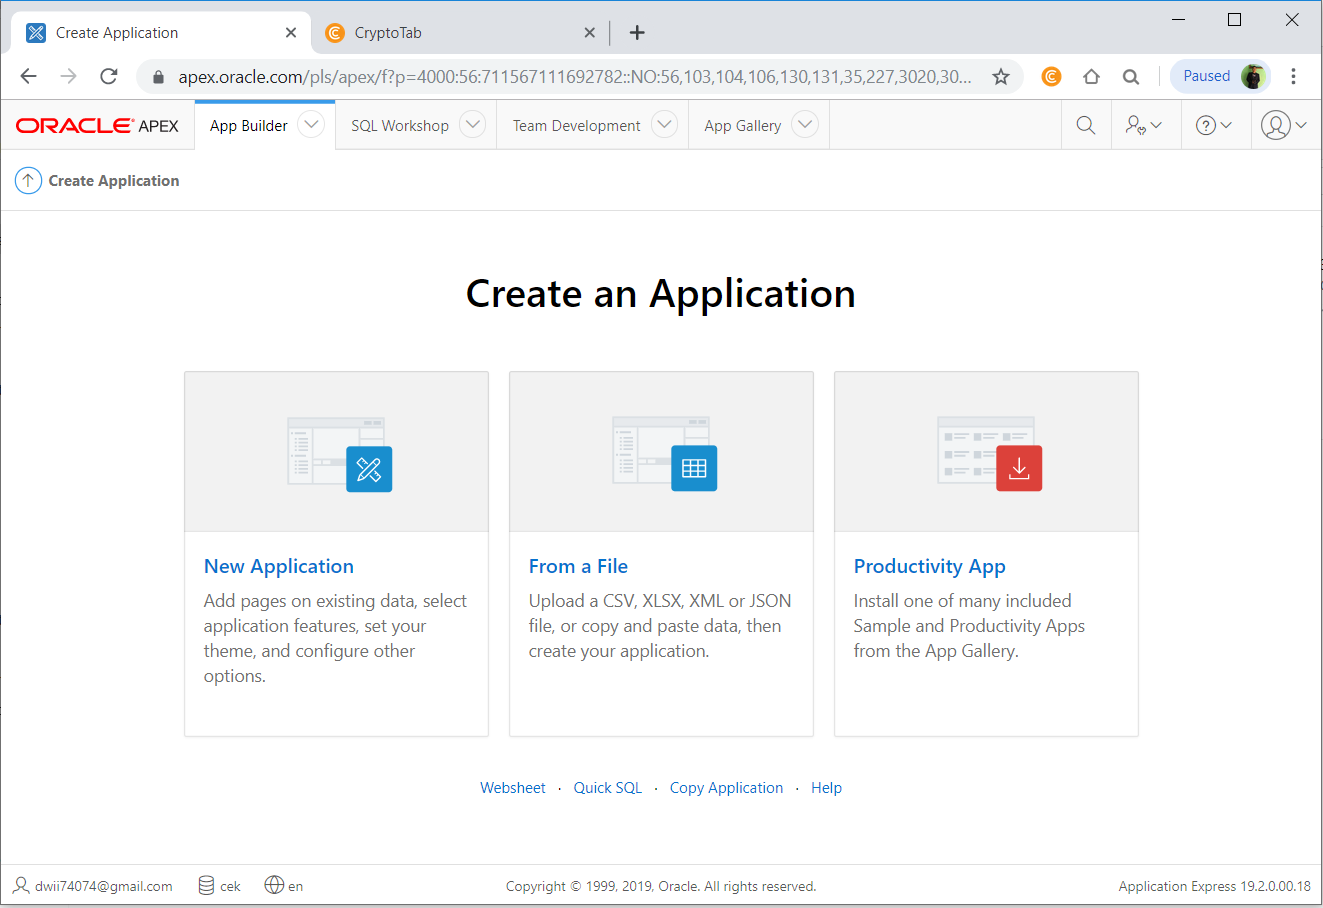
\includegraphics[scale=0.5]{gambar/4.PNG}
		\caption{Tampilan Klik Create}
\end{figure}
\\
\\
\\
\\
\\
\\
\\
\\
\\
\\
\\
\\
\\
\\
	\item setalah itu masuk dan klik form a file setelah itu masukkan data excell yg akan di buat.
	\begin{figure}[h]
	\centering
		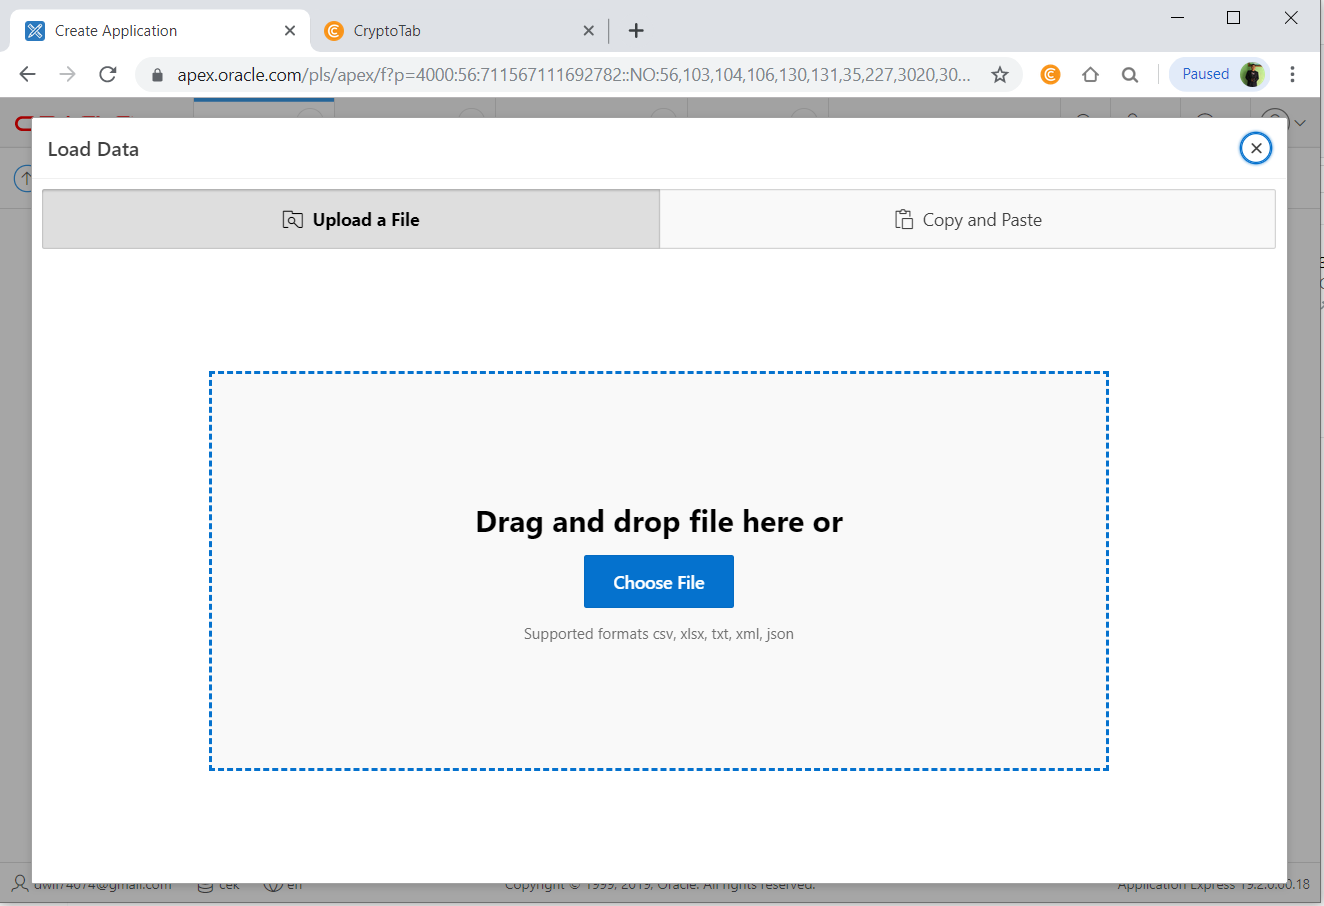
\includegraphics[scale=0.5]{gambar/5.PNG}
		\caption{Tampilan Form A File}
\end{figure}
\\
\\
\\
\\
\\
\\
\\
\\
\\
\\
\\
\\
\\
\\
\\
\\
\\
\\
\\
\\
\\
\\
\\

	\item Setalah masuk, isi table yang akan di buat dan pilih atau klik select sheet yang akan di buat
	\begin{figure}[h]
	\centering
		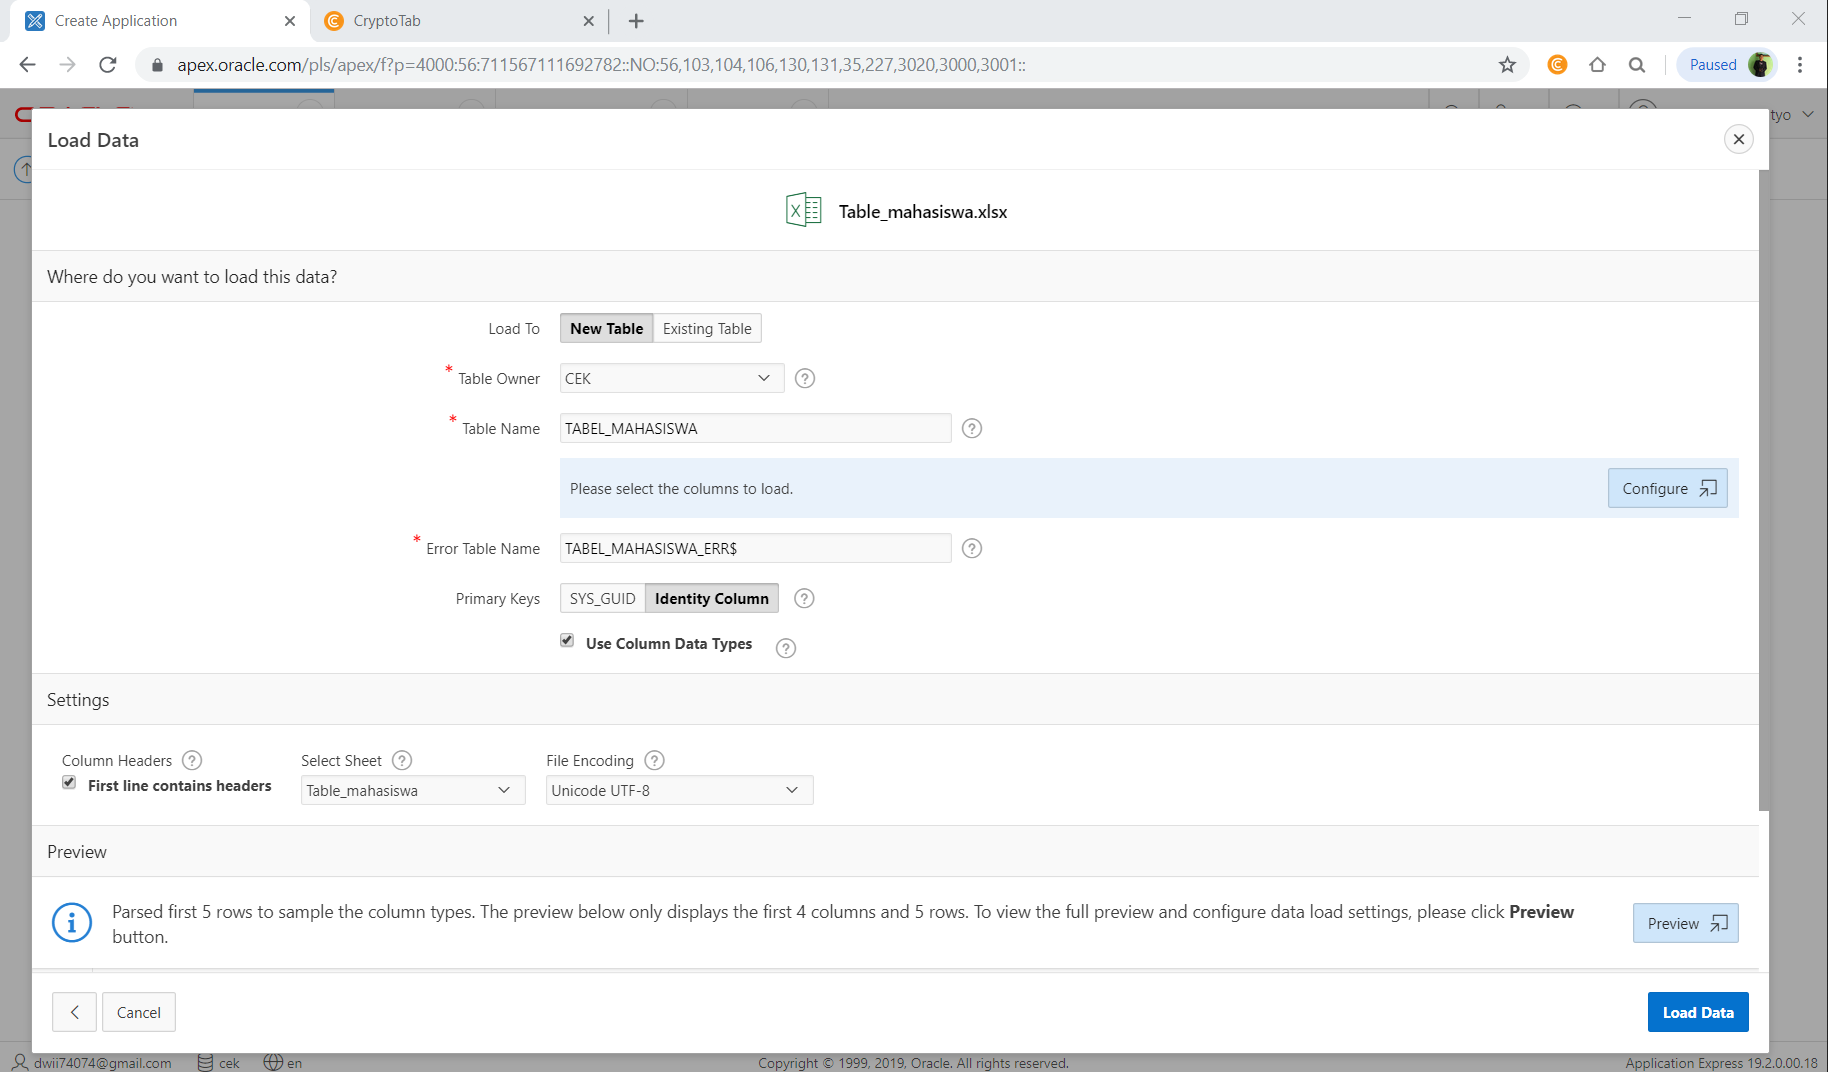
\includegraphics[scale=0.5]{gambar/6.PNG}
		\caption{Tampilan Klik Create}
\end{figure}
\\
\\
\\
\\
\\
\\
\\
\\
\\
\\
\\
\\
\\
\\
\\
\\

	\item setelah memasukkan data excell yang sudah di buat, kemudian cek config yang ada di bawah table nama dan akan muncul seperti ini
	\begin{figure}[h]
	\centering
		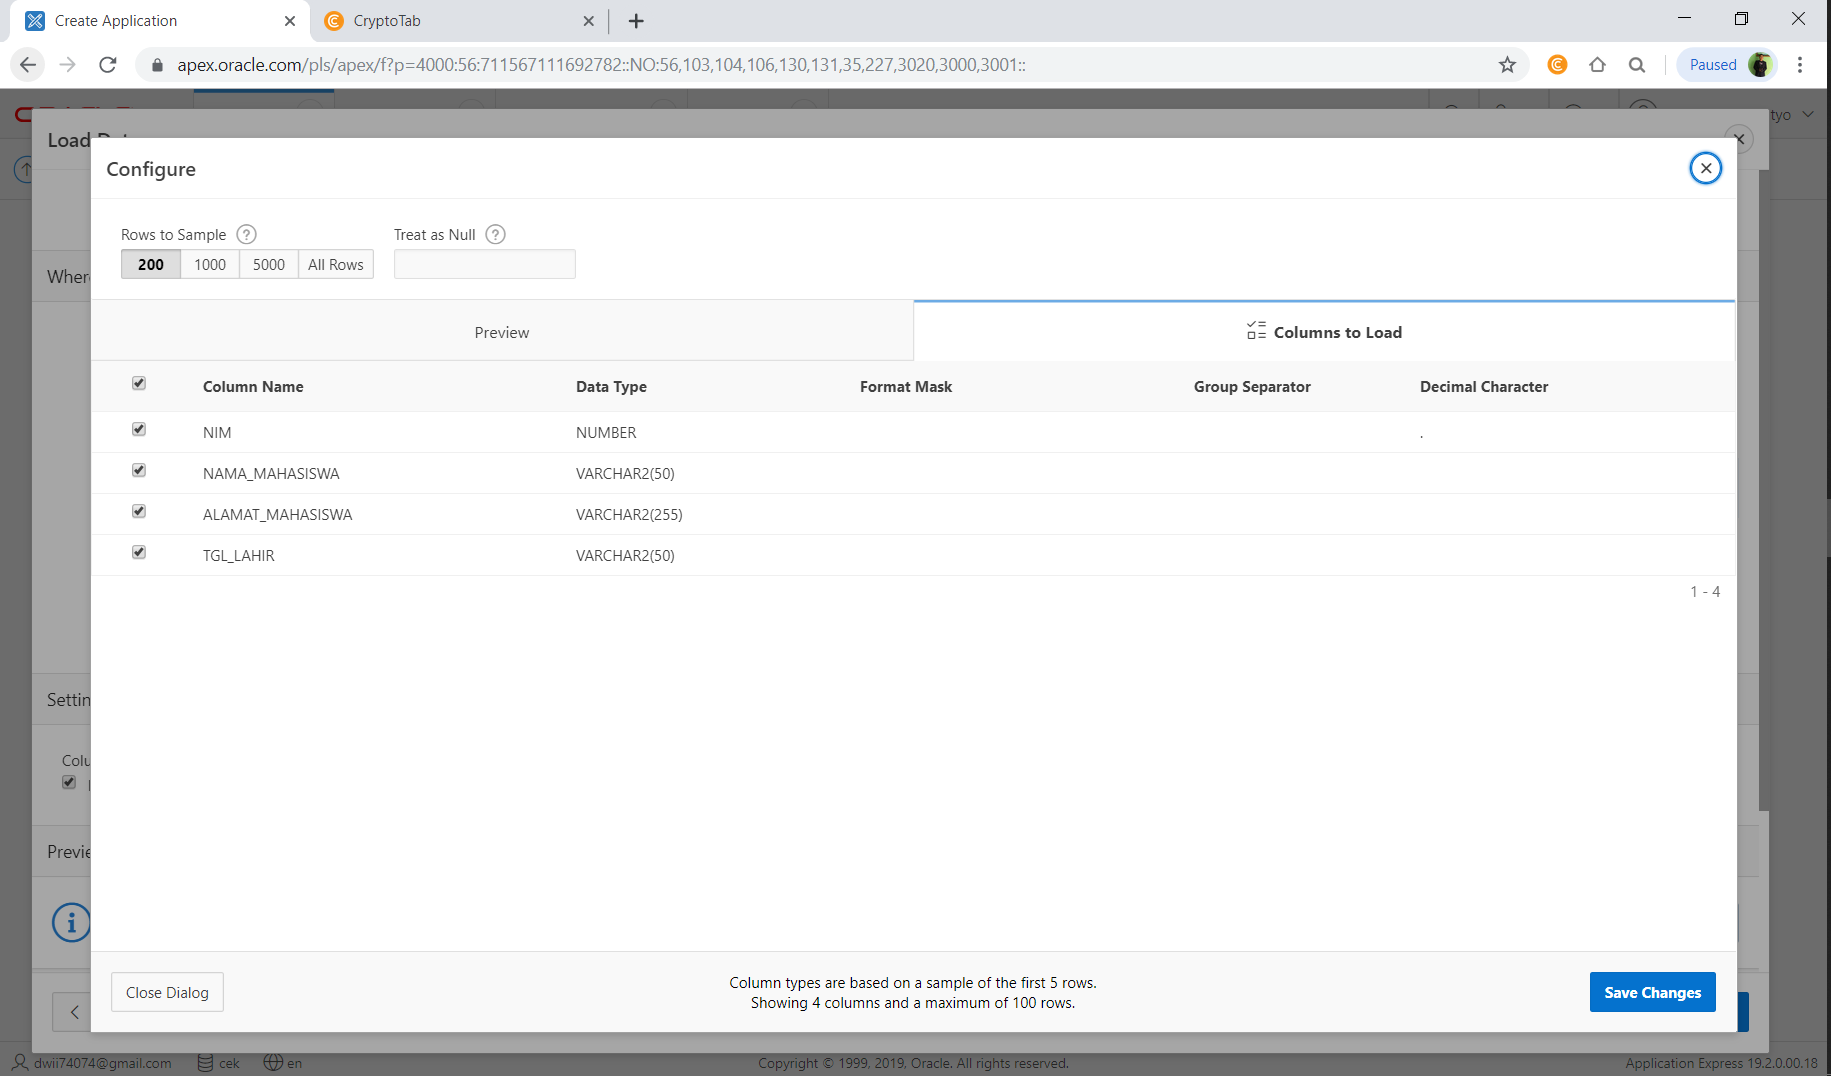
\includegraphics[scale=0.5]{gambar/7.PNG}
		\caption{Tampilan Cek Config}
\end{figure}
  \\
\\
\\
\\
\\
\\
\\
\\
\\
\\
\\
\\
\\
\\
\\
\\
	\item kemudan ikutin ke 4 data yang lain sesuai cara yang diatas
	\item setelah semua sudah diinputkan di APEX onliine, kemudian langsung menuju SQL Command dan menambahkan primary key dengan query berikut
	\begin{figure}[h]
	\centering
		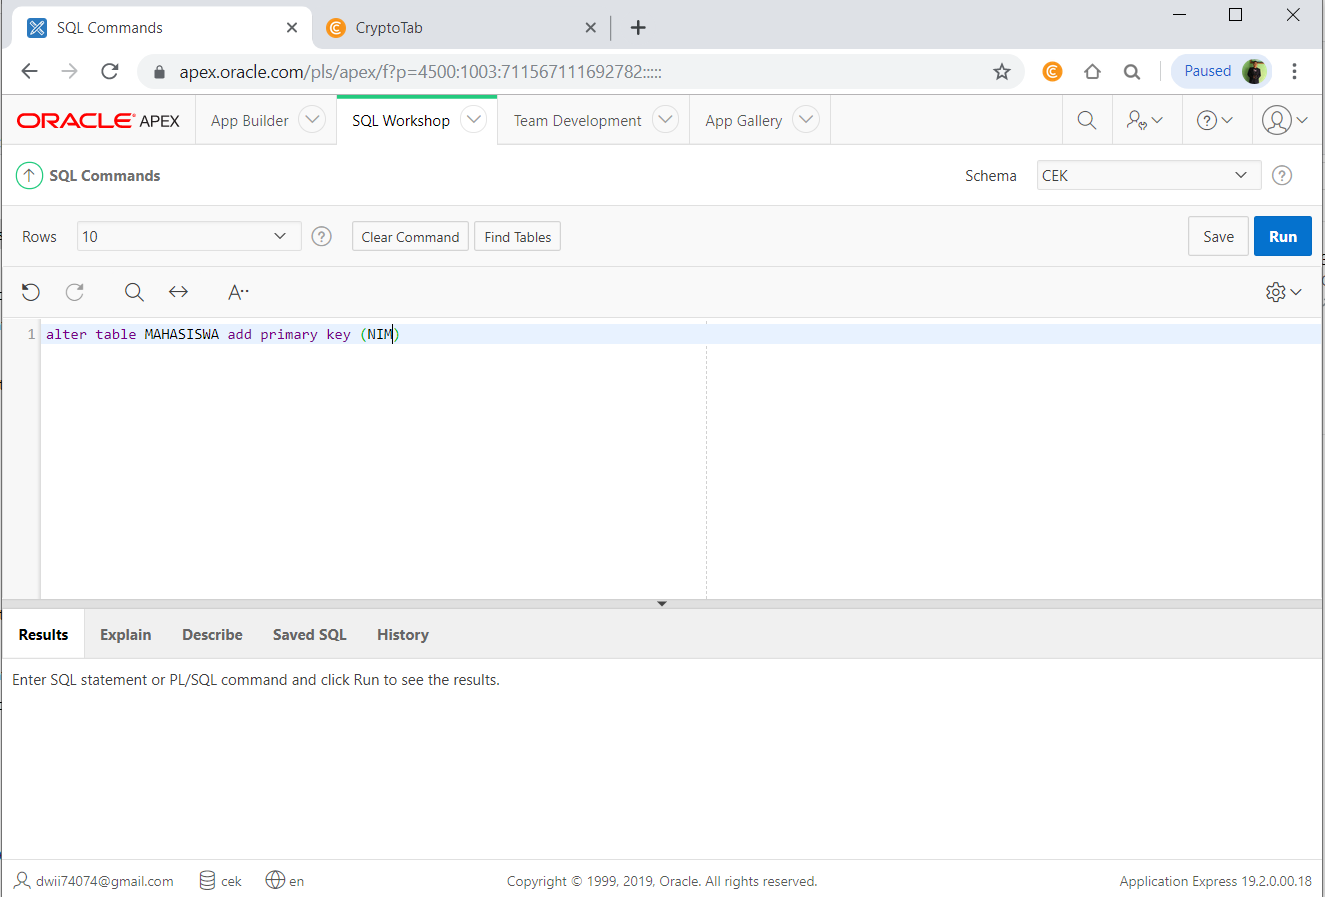
\includegraphics[scale=0.5]{gambar/9.PNG}
		\caption{Tampilan Query Primary Key}
\end{figure}
  \\
\\
\\
\\
\\
\\
\\
\\
\\
\\
\\
\\
\\
\\
\\
\\
	\item dan untuk menambahkan query foreign key dengan query sebagai berikut
	\begin{figure}[h]
	\centering
		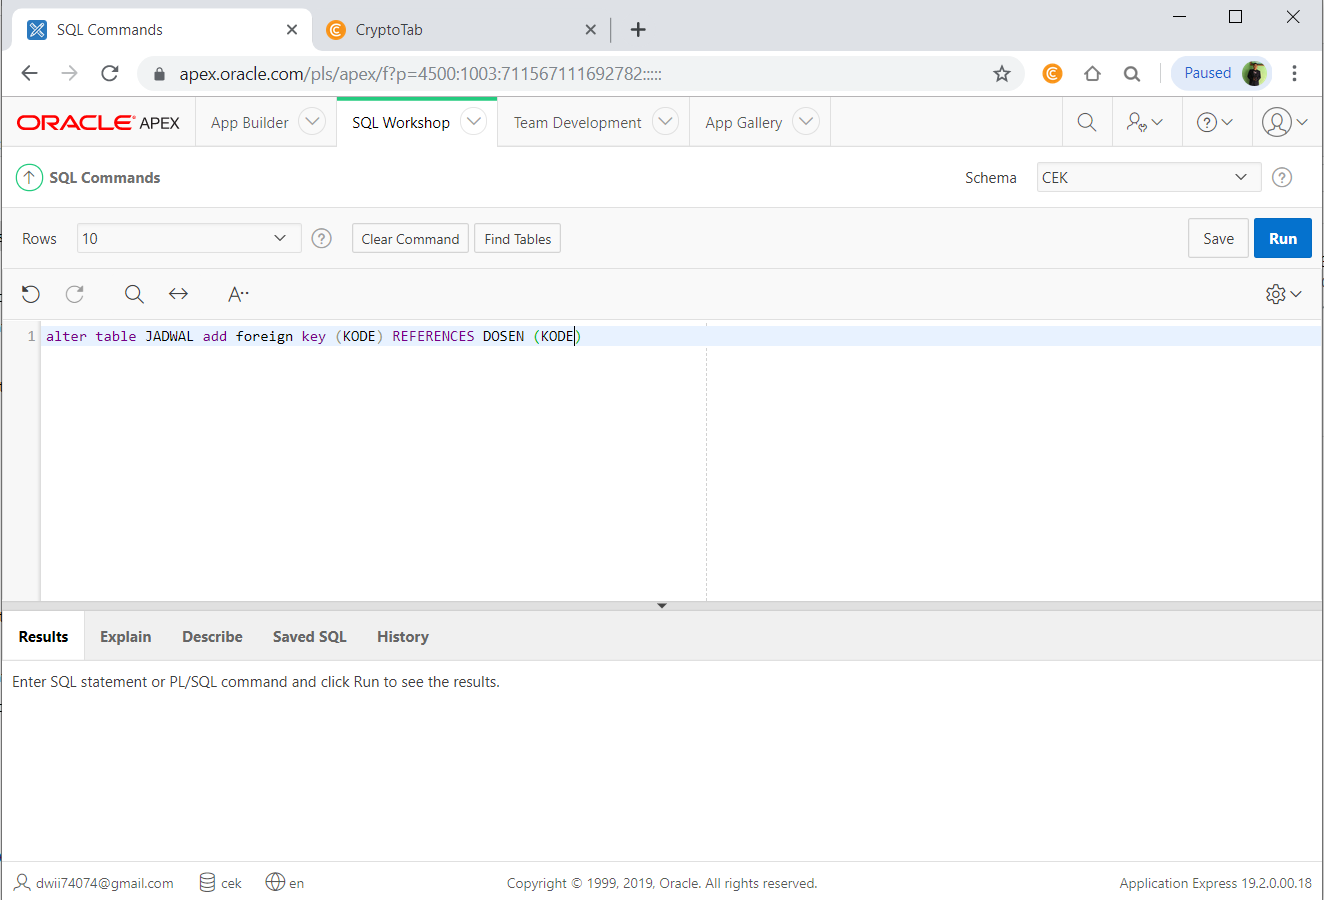
\includegraphics[scale=0.5]{gambar/10.PNG}
		\caption{Tampilan Query Foreign Key}
\end{figure}
	\item lakukan kesemua yg ingin di foreign key kan.
	\item setelah semua sudah selesai. langsung menuju App Builder dan akan tampil gambar seperti berikut
	\begin{figure}[h]
	\centering
		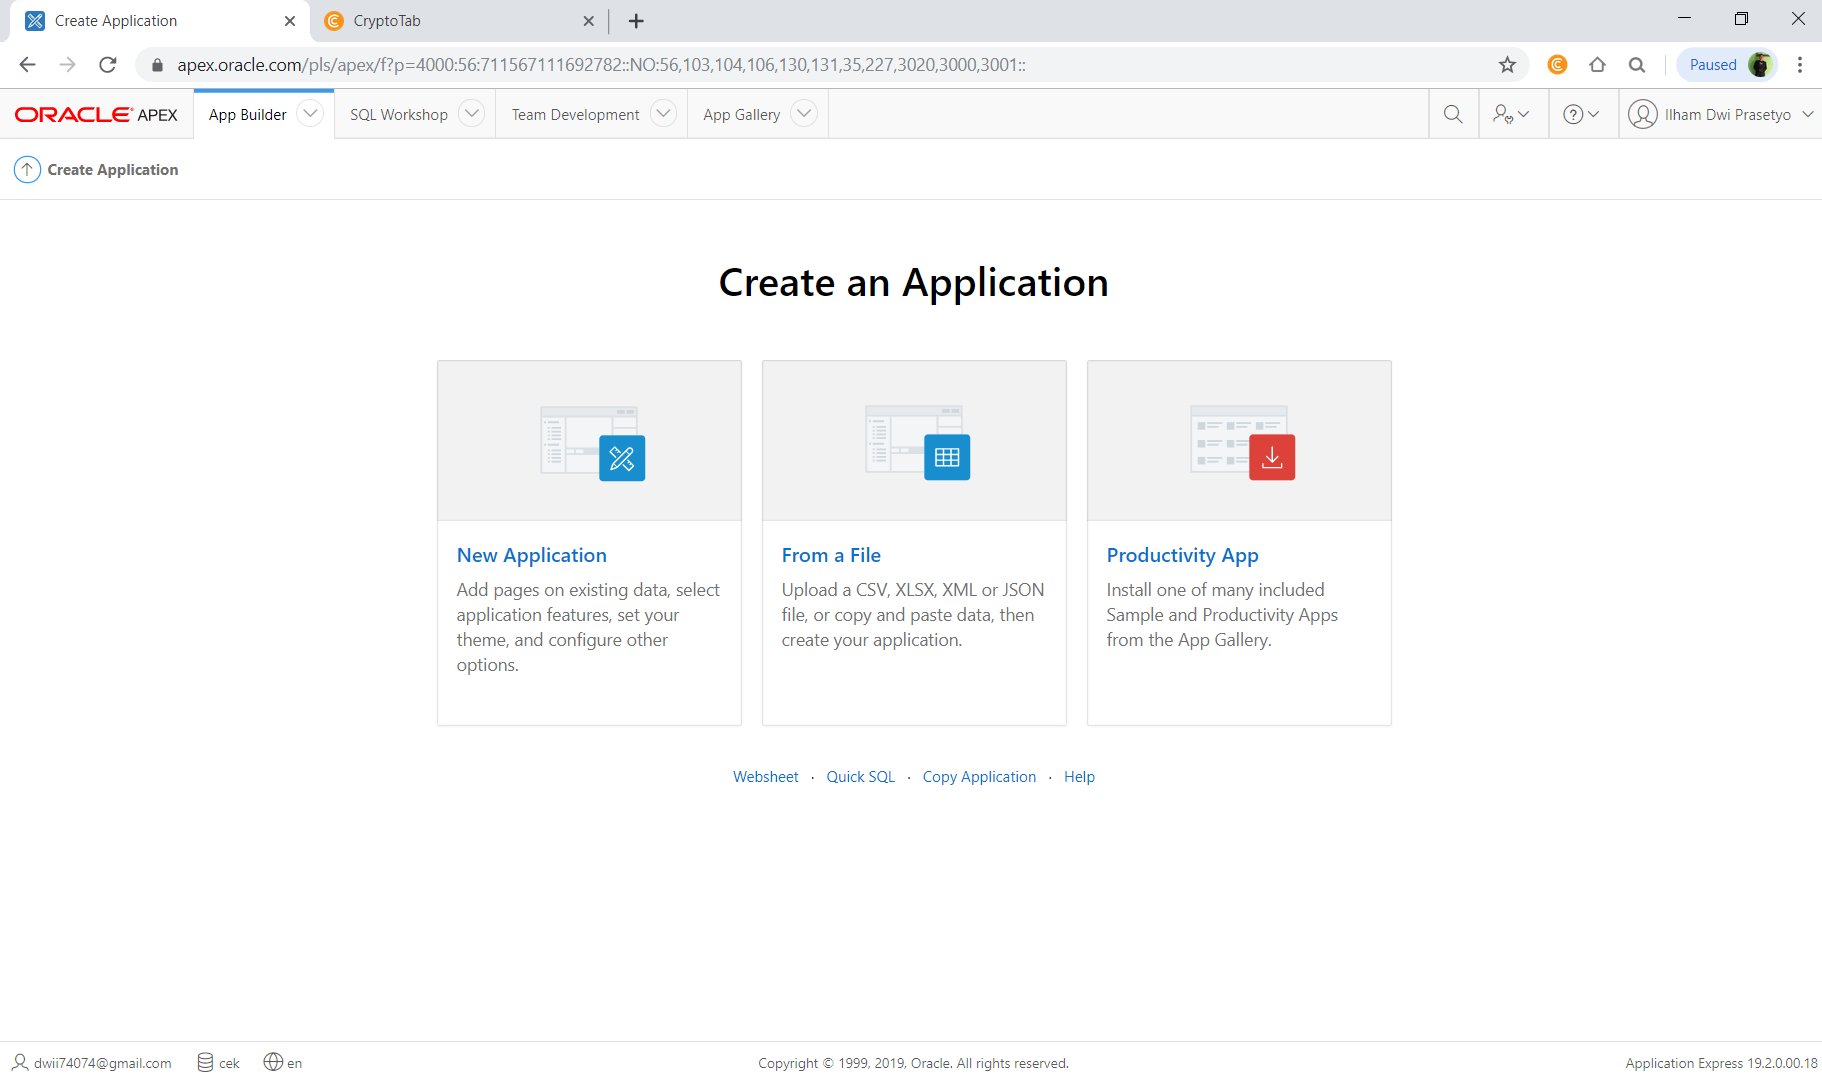
\includegraphics[scale=0.5]{gambar/11.PNG}
		\caption{Tampilan App Builder}
\end{figure}
 \\
\\
\\
\\
\\
\\
\\
\\
\\
\\
\\
\\
\\
\\
\\
\\
\\
\\
\\
\\
\\
	\item setalah muncul gambar tersebut, lalu klik New Application untuk lanjut menuju create app dan langsung pilih Interactive Report. akan muncul seperti berikut:
	\begin{figure}[h]
	\centering
		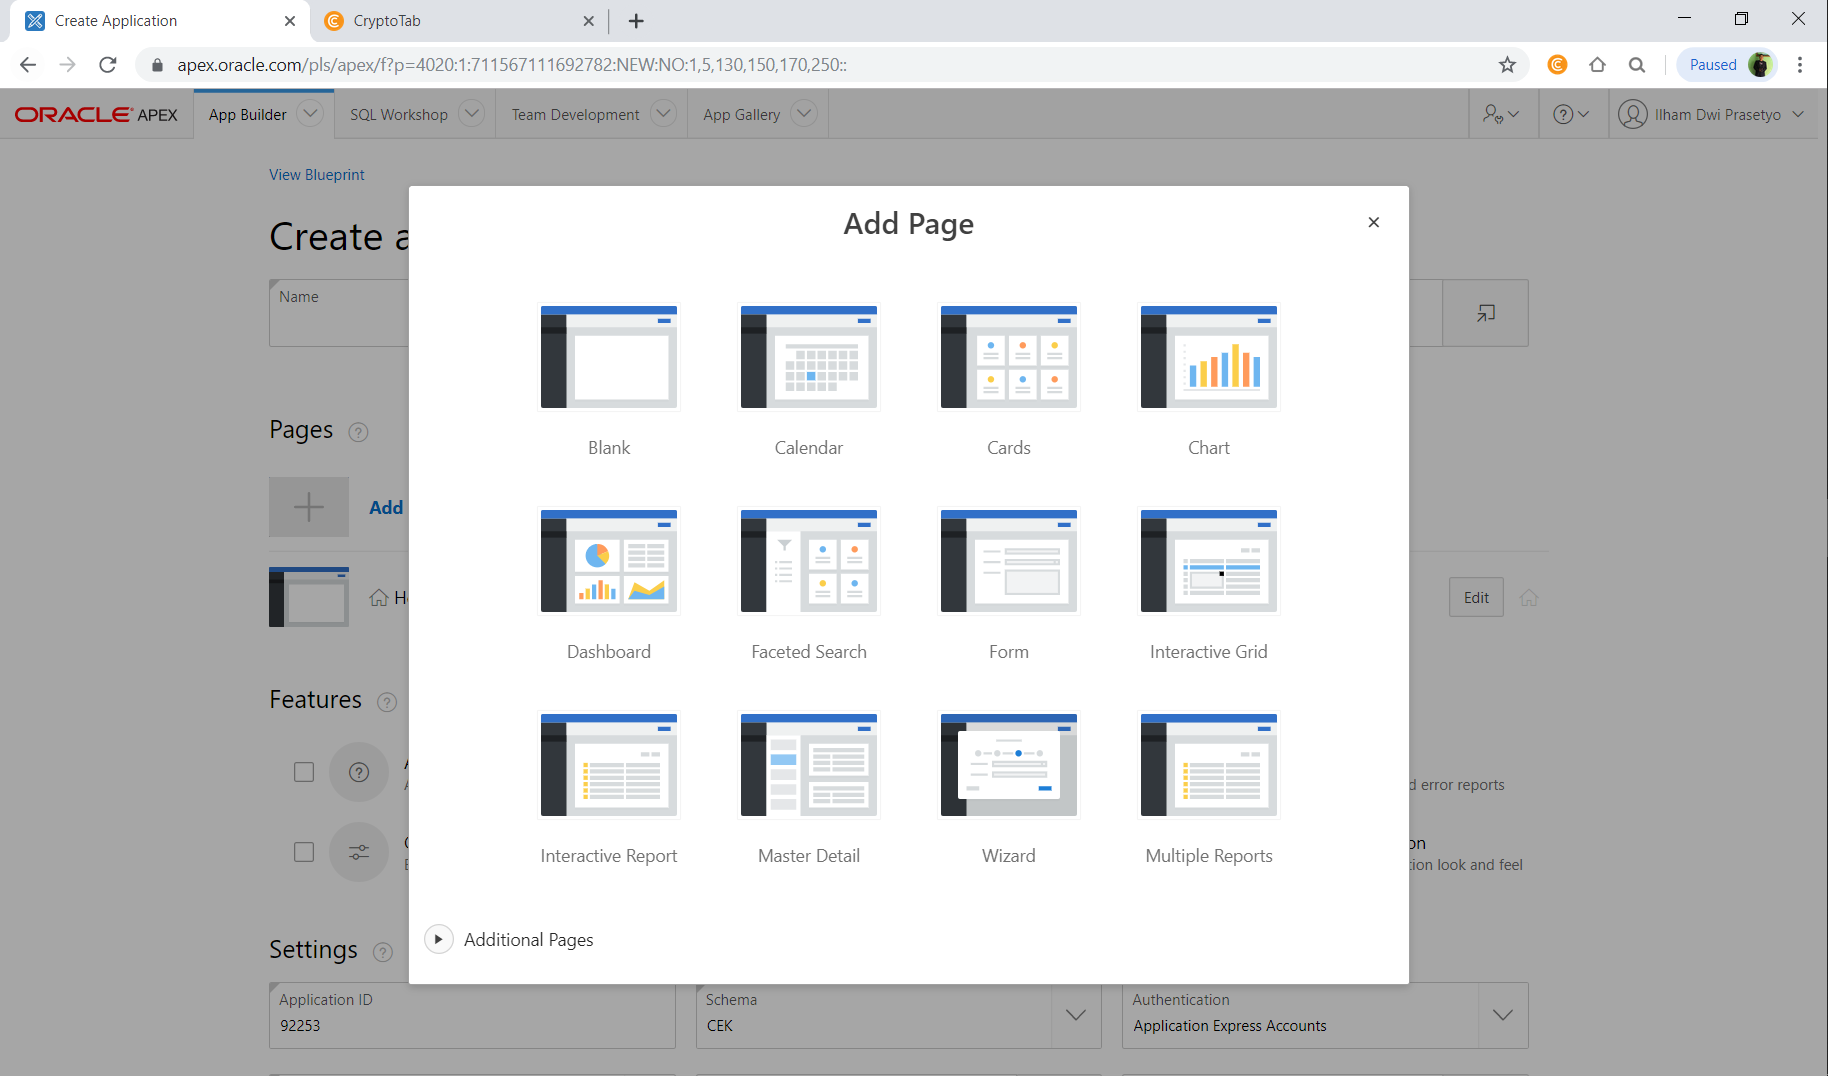
\includegraphics[scale=0.5]{gambar/12.PNG}
		\caption{Tampilan Pilihan Interactive Report}
\end{figure}
 \\
\\
\\
\\
\\
\\
\\
\\
\\
\\
\\
\\
\\
\\
\\
\\
\\
\\
\\
\\
\\
	\item setelah memilih interactive report, langsung add page untuk mengadd tabel tabel yang sudah di bikin dan ceklis include form.
	\begin{figure}[h]
	\centering
		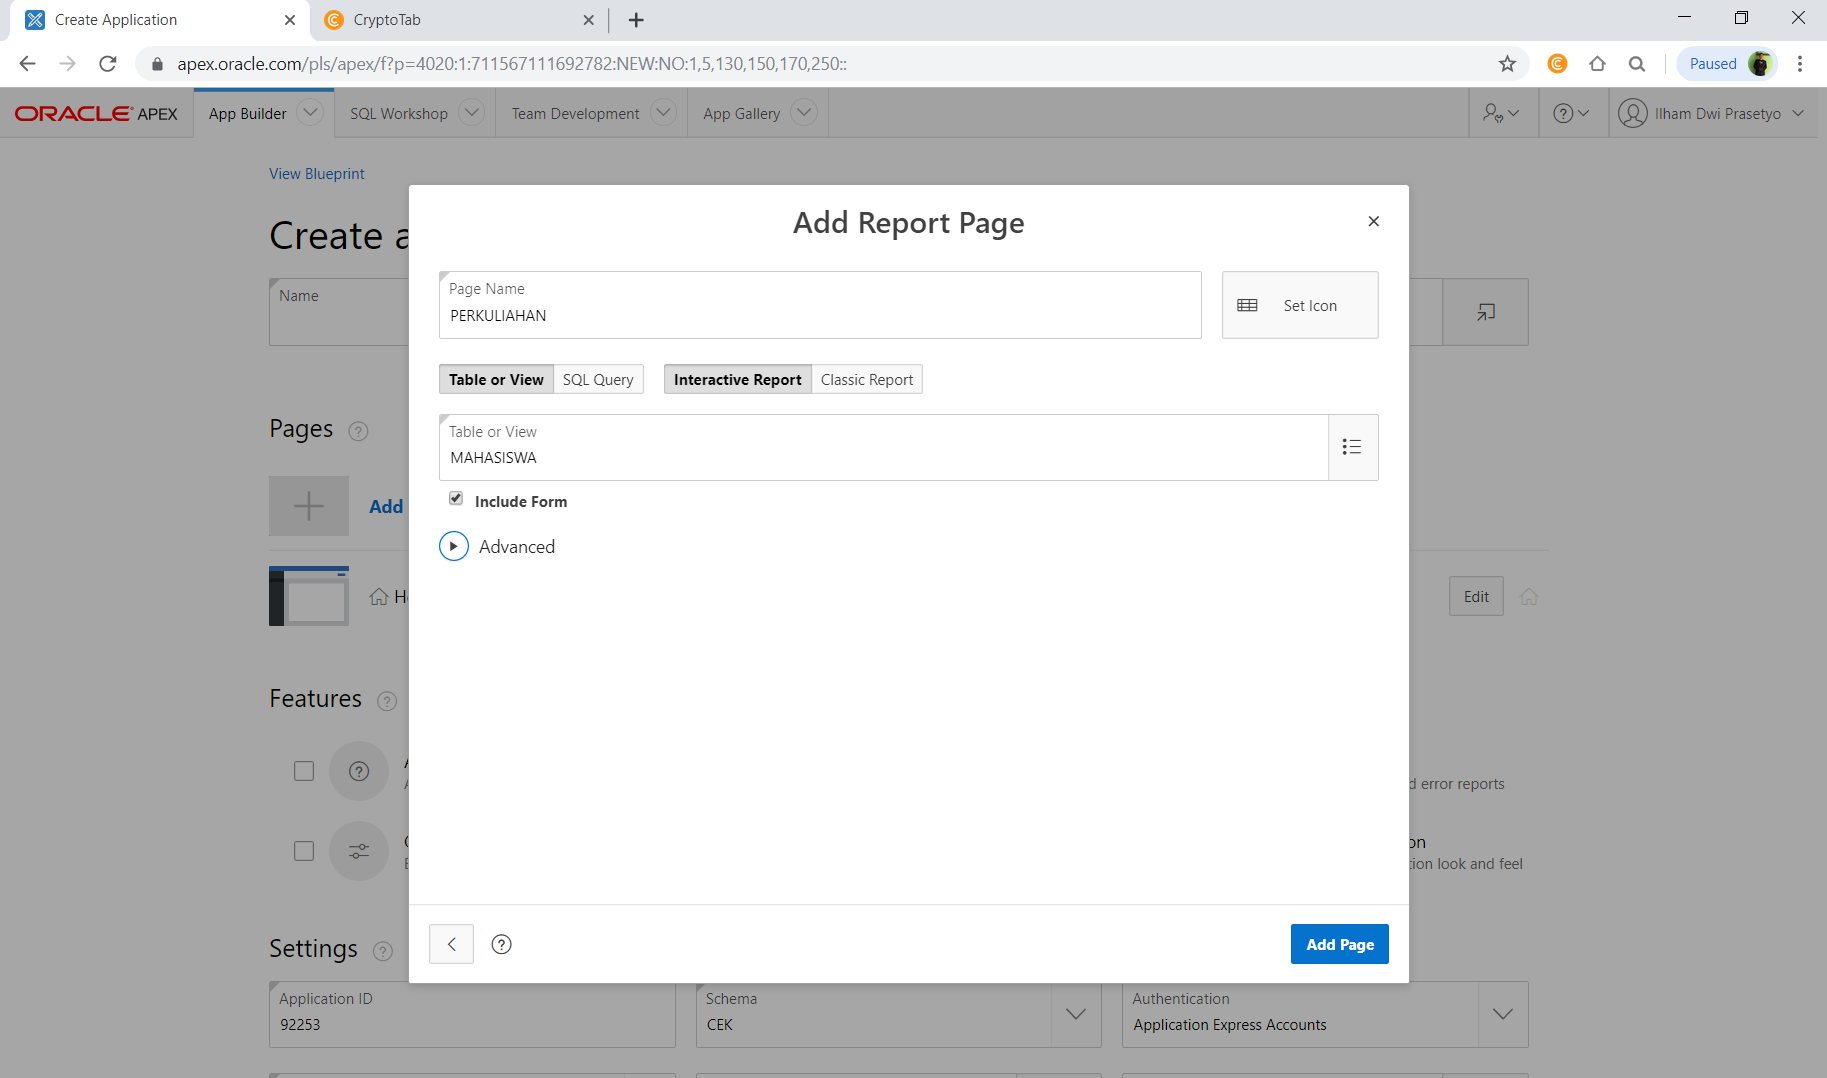
\includegraphics[scale=0.5]{gambar/13.PNG}
		\caption{Tampilan AddPage}
\end{figure}
 \\
\\
\\
\\
\\
\\
\\
\\
\\
\\
\\
\\
\\
\\
\\
\\
\\
\\
\\
\\
\\
	\item untuk tabel yang lain, sama saja caranya seperti yang diatas.
	\item dan setelah data tabel sudah di buat di page lalu klik Create App untuk melanjutkan ke pembuatan App
	 \begin{figure}[h]
	\centering
		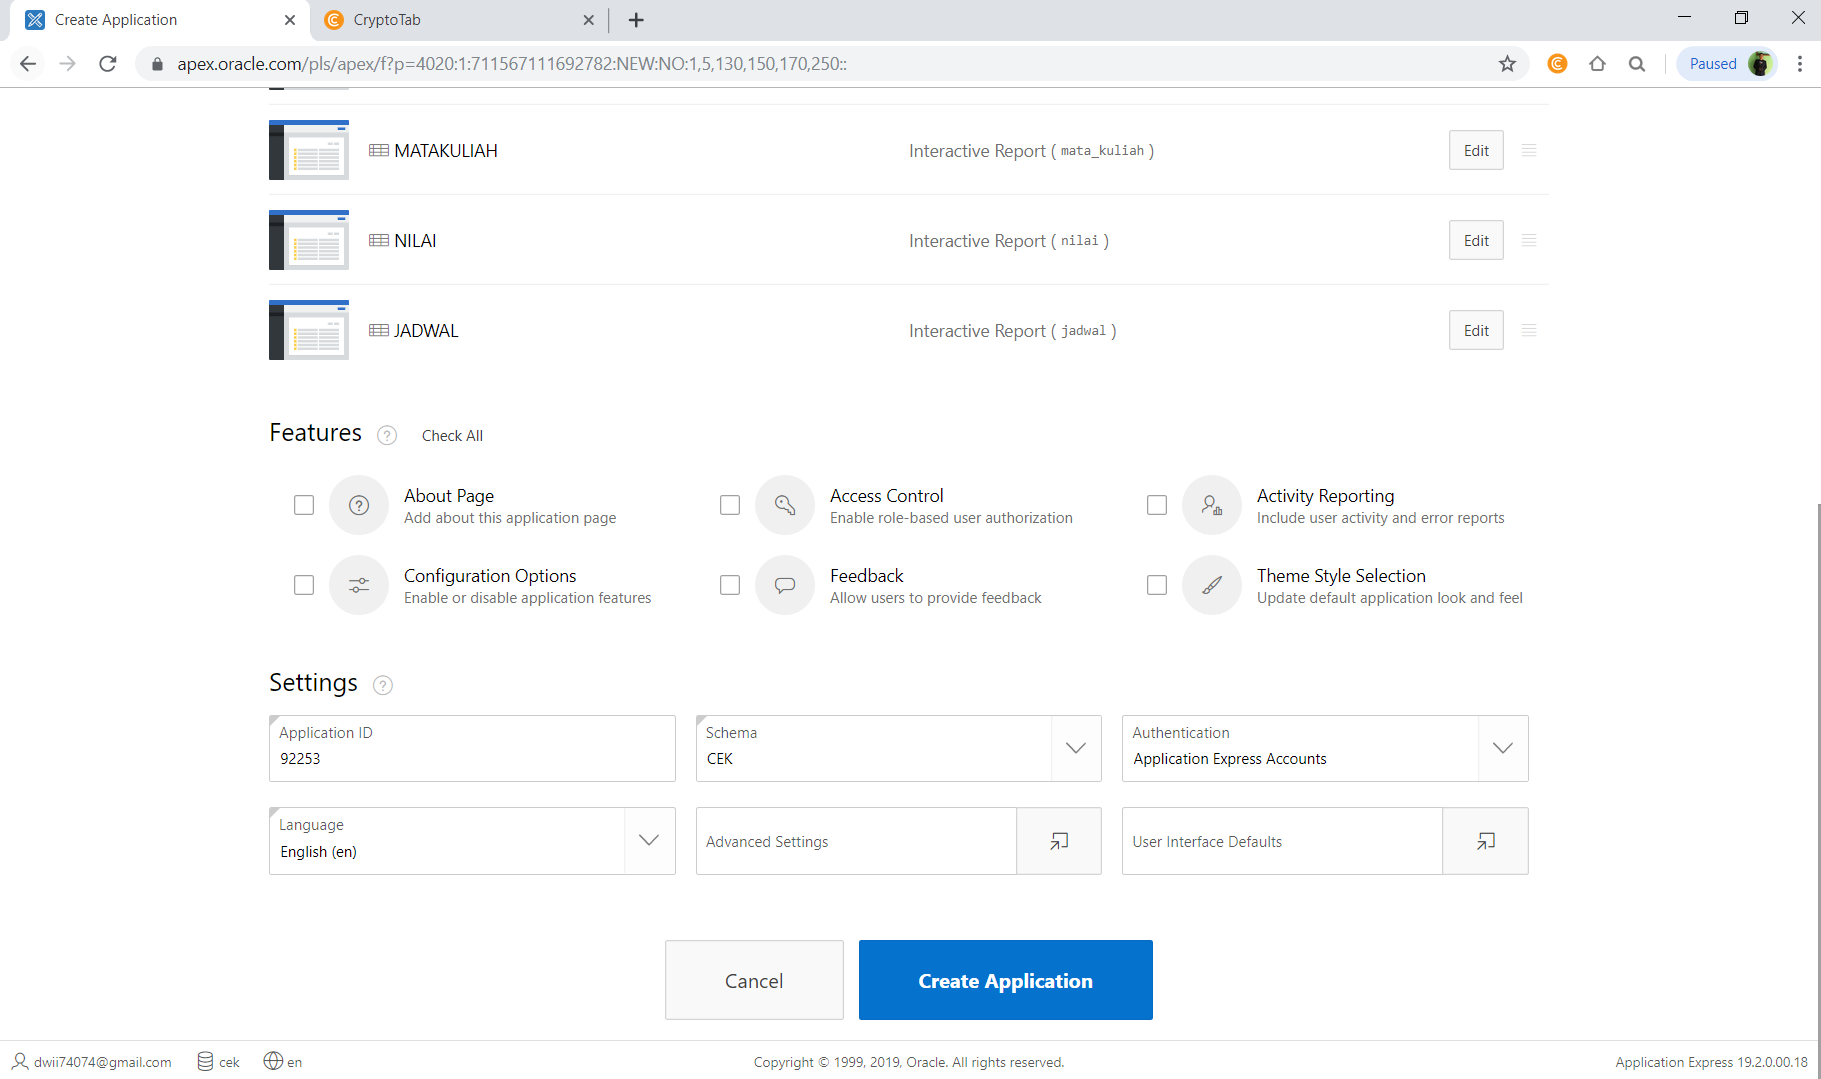
\includegraphics[scale=0.5]{gambar/14.PNG}
		\caption{Tampilan Klik Create App}
\end{figure}
\\
\\
\\
\\
\\
\\
\\
\\
\\
\\
\\
\\
\\
\\
\\
\\
\\
\\
\\
\\
\\
	\item tunggu hingga app berhasil dibuat
	\item setelah berhasil di buat akan menampilkan sebagai berikut
	 \begin{figure}[h]
	\centering
		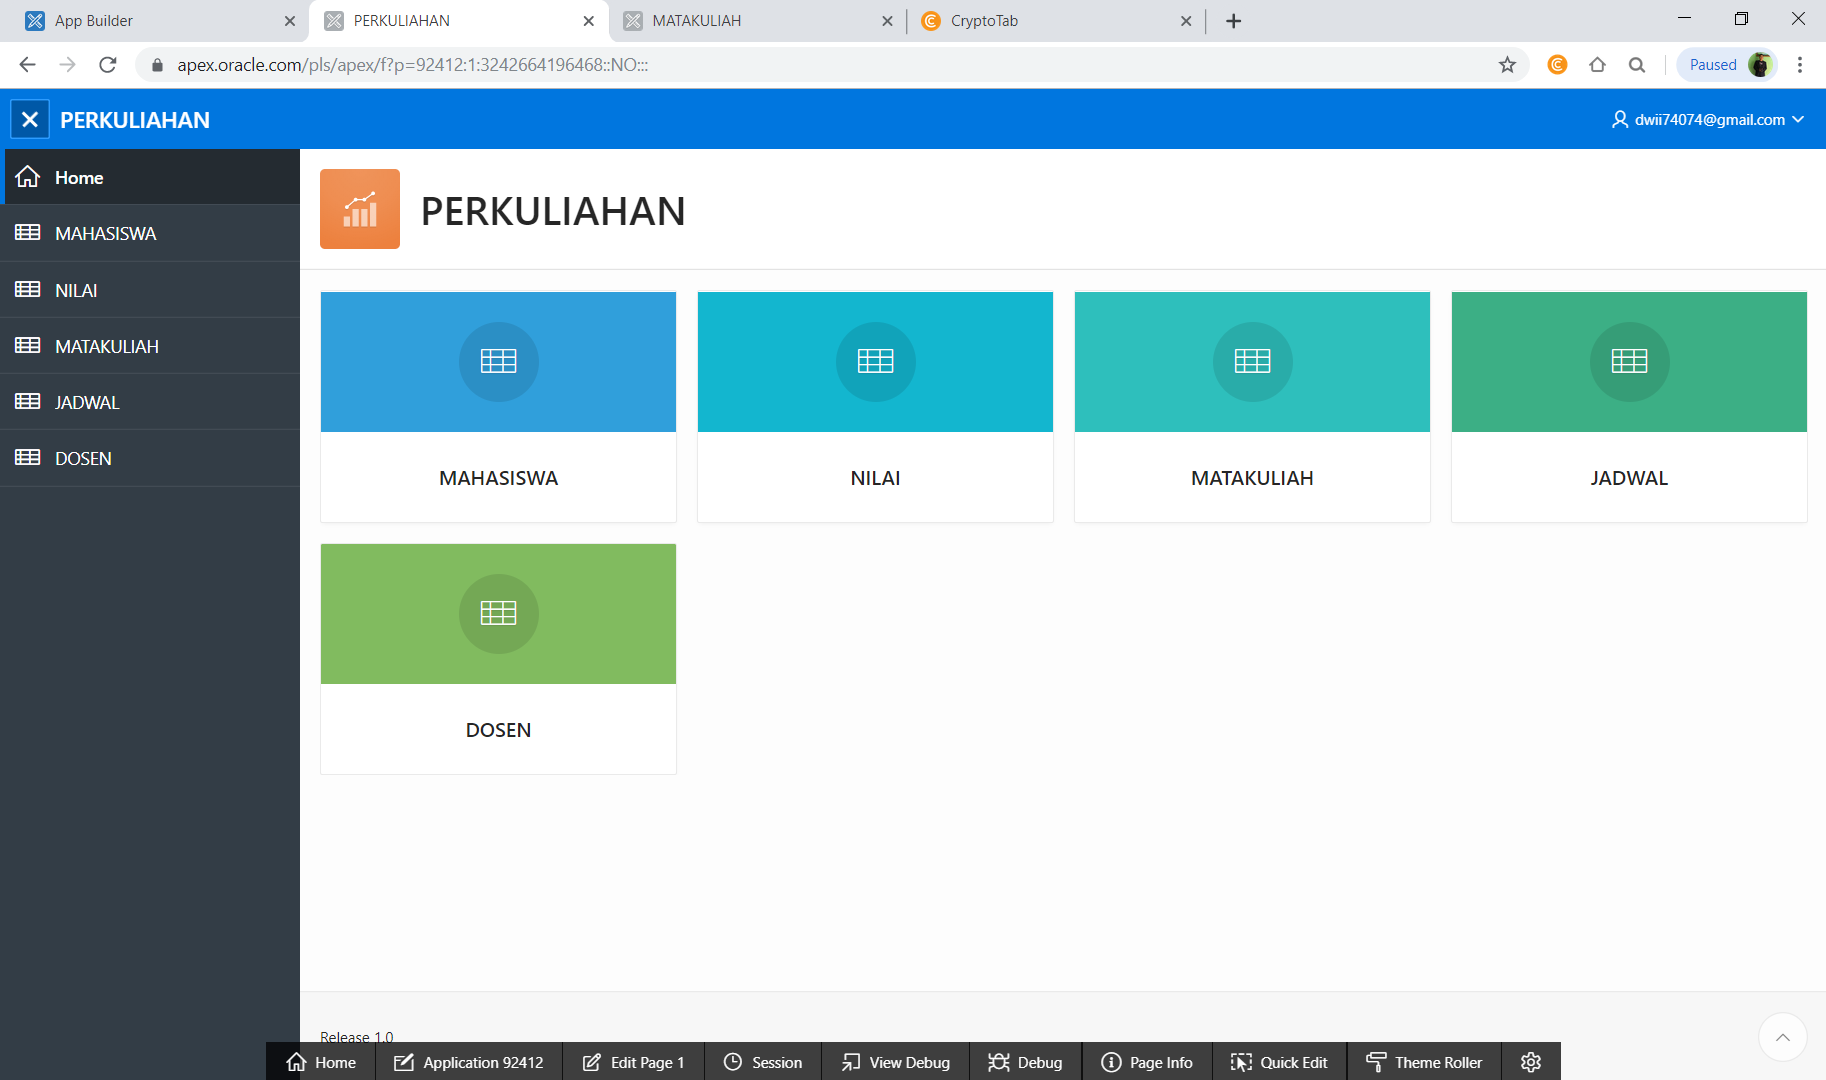
\includegraphics[scale=0.5]{gambar/15.PNG}
		\caption{Tampilan Tampilan App yang sudah berhasil}
\end{figure}

\section{LINK}
Link : https://apex.oracle.com/pls/apex/f?p=92412:1:711567111692782:::::
Username :dwii74074@gmail.com\\
Password :ilhamdwi170214\\
      \end{enumerate}
      
       

\end{document}
